\documentclass[a4paper,12pt]{article}
\usepackage{amsfonts,amsmath,amssymb,anysize}
\usepackage{bibentry,blindtext,braket,cancel}
\usepackage{fancyhdr,graphicx}
\usepackage{listings,multicol,mathtools}
\usepackage{pdfpages,siunitx,verbatim}
\usepackage{xfrac,xcolor}

\marginsize{1.5cm}{1.5cm}{1cm}{1cm}
\linespread{1.5}

\pagestyle{fancy}
\fancyhf{}
\lhead{Phys. 310 Quantum Mechanics and Its Applications I (Term 212)}
\rhead{Formula Sheet}

\begin{document}
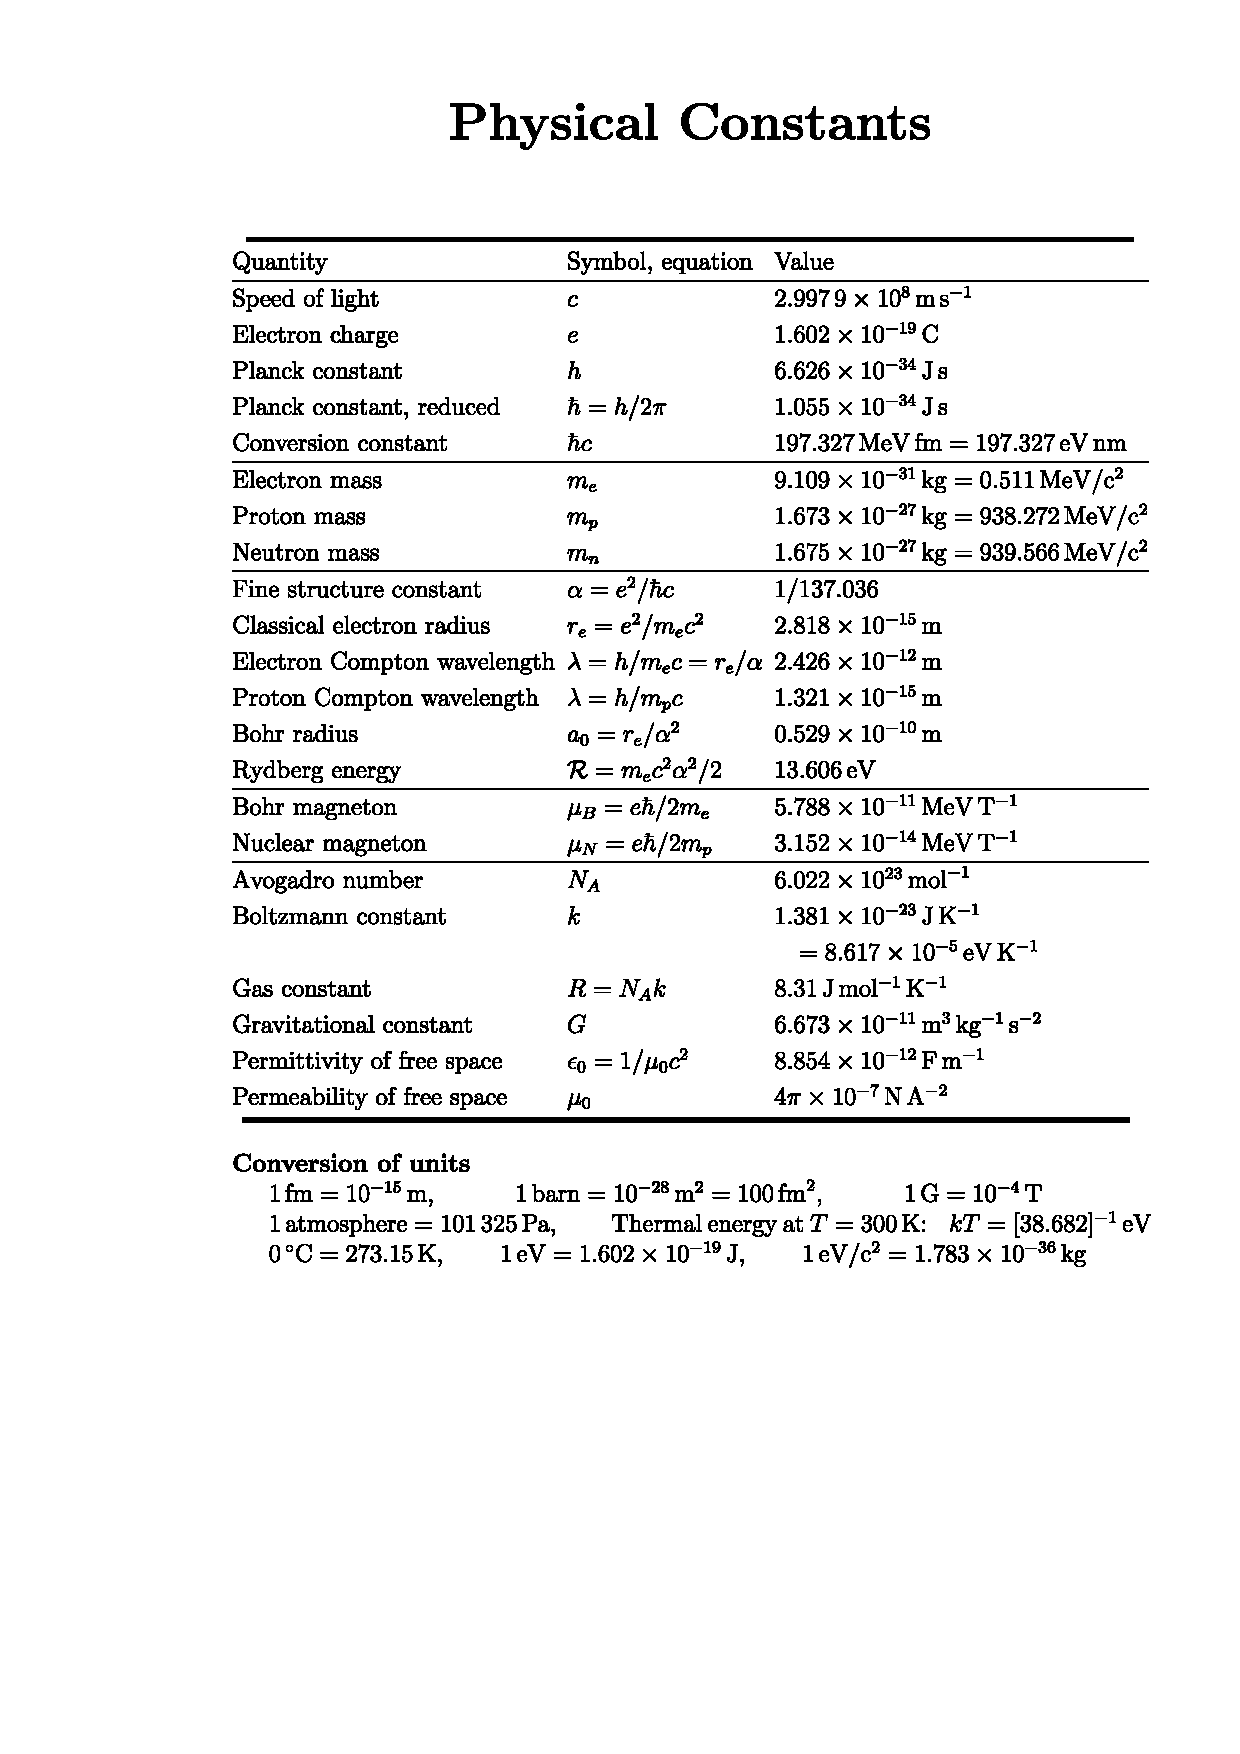
\includepdf{Constants.pdf}
\begin{center}\textbf{\underline{\huge{Formula Sheet}}}\end{center}
\subsection*{\underline{Properties of the Solution of 1D stationary Schrodinger Equation:}}
\begin{enumerate}
\item For 1D potential, all stationary solutions are non-degenerate.
\item Stationary square integrable solution exist only for $E > min{V(x)}$ 
\item If V(x) is real, then $\Psi$(x) can be taken to be real.
\item Eigenvalues of a Hermitian Hamiltonian are all real.
\item The eigenfunctions of a Hermitian operator form a complete orthogonal basis set, for smooth potentials.
\item 1D Schrodinger equation Solution is real up to an over all phase.
\item For a given 1D even potential the stationary states are either even or odd.
\item The wave function and its first order space derivative is continuous all over space and in particular at the boundaries of a finite potential.
\item At boundaries with Dirac delta function potential, the first space derivative of the wavefunction is discontinuous. 
\item Physical solution should be finite all over space, no blow ups, in particular at infinity.
\item The number of nodes (zeros) of the eigenfunction increases by one unit as we move from the ground state (zero nodes) to higher excited states.
\item Bound states exist only for confining potential (classically between turning points of the potential).
\end{enumerate}
\subsection*{\underline{The Origin of Quantum Physics:}}
\begin{align}
    &E=h\omega
    &p=\frac{h}{\lambda}=\hbar k
    &\\
    &\lambda=\frac{h}{p}
    &\lambda_C = \frac{h}{mc}
\end{align}
\subsection*{\underline{Blackbody Radiation:}}
Plank energy spectral density: \resizebox{.4\hsize}{!}{$\rho(\nu)=\frac{8\pi h \nu^3}{c^3}\left[ \frac{1}{\exp \left(\frac{h\nu}{k_BT} \right)-1} \right]$}
\vspace{0.3cm}
\hrule
\subsection*{\underline{Photoelectric Effect:}}
$W$ is the work function of irradiated metal. $V_s$ is the stopping potential.
$$K=\sfrac{1}{2}\ mv^2=h\nu-W=\frac{hc}{\lambda}-W\ ;\quad K=\sfrac{1}{2}\ mv^2=|e|V_s\leftrightarrow V_s=\frac{K}{|e|}$$
$$\nu\geq\frac{W}{h}=\nu_{\min};\quad \nu=\frac{1}{T}=\frac{c}{\lambda};\quad \nu=\frac{\omega}{2\pi}$$
% \vspace{0.3cm}
\hrule
\subsection*{\underline{de Broglie Formula:}}
$$\lambda=\frac{h}{p}=\frac{h}{mv}$$
\vspace{0.3cm}
\hrule
\subsection*{\underline{Bohr Hydrogen-like Atom:}}
\begin{align*}
    &E_n=-\frac{Z^2}{n^2}R&\ &\quad R=13.6\,\unit{\electronvolt}\\
    &r_n=\frac{a_0}{Z}n^2&\ &\quad a_0=0.53\times10^{-10}\,\unit{\metre}\\
    &h\nu=E_n-E_m=Z^2R\left( \frac{1}{m^2}-\frac{1}{n^2} \right)&\ &\quad n>m
\end{align*}
\subsection*{\underline{The Wave Function:}}
$\Psi(x,t)$ obeys Schrodinger's equation, and the normalization condition $\int_{-\infty}^\infty |\Psi(x,t)|^2dx=1$:
\begin{equation}
    \braket{x}=\int_{-\infty}^\infty x|\Psi(x,t)|^2dx;
    \braket{p}=\int_{-\infty}^\infty \Psi^*(x,t)\frac{\hbar}{i}\frac{\partial}{\partial x}\Psi(x,t)dx;
    \braket{Q(\hat{x},\hat{p})}=\int_{-\infty}^\infty \Psi^*(x,t)Q\left( x,\frac{h}{i} \frac{\partial}{\partial x} \right)\Psi(x,t)dx
\end{equation}
\begin{flalign}
    &i\hbar \frac{\partial }{\partial t}\Psi(x,t)=H\Psi(x,t);
    &&\Psi(x,t)=\psi(x)e^{-iEt/\hbar};
    &&H\psi(x)=E\psi(x)
    &\\
    &\rho(x,t)=|\Psi(x,t)|^2;
    &&\frac{\partial}{\partial t}\rho(\textbf{x},t)+\nabla \cdot \textbf{J}(\textbf{x},t)=0;
    &&J(x,t)=\frac{i\hbar}{2m}\left( \Psi\frac{\partial \Psi^*}{\partial x}-\Psi^*\frac{\partial \Psi}{\partial x} \right)
    &\\
    & \mathbf{J}(\mathbf{x},t)=\frac{h}{2im}\left( \psi^*\nabla\psi-\psi\nabla\psi^* \right)
    &&p=\frac{\hbar}{i}\nabla;
    &&[x_i,p_j] = i\hbar \ \delta_{i,j}
\end{flalign}
% A Hermitian operator $Q$ obey: $\int\psi^*(x)Q\psi(x)\,dx=\int(Q\psi(x))^*\psi(x)\,dx$, and $Q^\dagger = Q$.\\
Hermitian conjugate $A^\dagger$ is defined by: $\int(A\psi(x))^*\psi(x),dx=\int\psi(x)A^\dagger\psi(x),dx$.
\subsection*{\underline{Fourier Transform}}
\begin{flalign}
    &\Psi(x)=\frac{1}{\sqrt{2\pi}}\int dk\Phi(k)e^{ikx},
    &&\Phi(k)=\frac{1}{\sqrt{2\pi}}\int dx\Psi(x)e^{-ikx}
    &&\int dx|\Psi(x)|^2 = \int dk|\Phi(k)|^2
    &\\
    &\Psi(x)=\frac{1}{(2\pi)^\frac{3}{2}}\int d^3k\Phi(\textbf{k})e^{i\textbf{k}\cdot \textbf{x}},
    &&\Phi(k)=\frac{1}{(2\pi)^\frac{3}{2}}\int d^3x\Psi(\textbf{x})e^{-i\textbf{k}\cdot \textbf{x}}
    &&\int d^x|\Psi(\textbf{x})|^2 = \int d^k|\Phi(\textbf{k})|^2
    &\\
    &\frac{1}{2\pi} \int_{-\infty}^\infty e^{ikx}dx = \delta(k)
    &&\frac{1}{(2\pi)^3} \int_{-\infty}^\infty e^{i\textbf{k}\cdot \textbf{x}}d^3x = \delta^{(3)}(k)
    &&\Psi(x,t)=\frac{1}{(2\pi)^3}\int\phi(k)e^{i(\mathbf{k}\cdot\mathbf{x}-\omega(\mathbf{k})t)}\,dk^3
\end{flalign}
\subsection*{\underline{Wavepackets}}
\begin{equation}
    v_{group} =\frac{d\omega}{dk};\  \Delta k\Delta x \simeq 1
\end{equation}
\subsection*{\underline{Complete Basis Set:}}
Given that $H\psi_n(x)=E_n\psi_n(x);\quad \int\phi^*_n(x)\phi_m(x)dx=\delta_{nm}$, where $\{\phi_n\}$ is a complete set, then:
\begin{align}
    \psi(x)&=\sum_nc_n\phi_n(x);\quad C_n=\int\psi^*_n(x)\psi(x)\,dx\\
    \int\psi^*(x)\psi(x)dx&=\sum_n|c_n|^2=1\\
    E&=\int\psi^*_n(x)H\psi_m(x)dx=\sum_n|c_n|^2E_n\\
    \Psi(x,0)&=\psi(x)=\sum_nc_n\phi_n(x)\implies\Psi(x,t)=\sum_nc_ne^{-iE_nt/\hbar}\phi_n(x)\\
    c_n&=\int\phi_n^*\Psi(x,0)dx
\end{align}
\subsection*{\underline{Commutator Properties:}}
\begin{equation}
[A,A]=0;\quad
[A,B]=-[B,A];\quad
[A+B,C]=[A,C]+[B,C]\quad
\end{equation}
\begin{equation}
[AB,C]=[A,C]B+A[B,C];\quad
[A,BC]=[A,B]C+B[A,C];\quad
\end{equation}
\begin{equation}
[A,[B,C]]+[B,[C,A]]+[C,[A,B]]=0
\end{equation}
\subsection*{\underline{Uncertainty Principle:}}
\begin{align}
    &(\Delta Q)^2 = \braket{Q^2} - \braket{Q}^2 = \braket{(Q-\braket{Q})^2}
    &\Delta x \Delta p \geq \frac{\hbar}{2}
\end{align}
Where $\Delta Q$ is the uncertainity for the Hermitian Operator Q.
\subsection*{\underline{Operators:}}
For the operator $\hat{A}$, $\hat{A}\psi=a\psi$. $a$ in an eigenvalue and $\psi$ is an eigenfunction of $A$. Then, the following properties hold:
\begin{itemize}
    \item $\hat{A}^n\psi=a^n\psi,\quad \hat{A}^{-1}\psi=a^{-1}\psi,\quad e^{i\hat{A}}\psi=e^{ia}\psi,\quad F(\hat{A})\psi=F(a)\psi$
    \item $\hat{A}^{\dagger}=A,\ \hat{A}\ket{\phi_n}=a_n\ket{\phi_n} \quad \implies a_n\in \mathbb{R}, \braket{\phi_m|\phi_n}=\delta_{mn}$
    \item If $\{\phi_n\}$ is a complete and orthonormal for a Hermitian operator, then the operator is diagonal in the eigenbasis, $\{\phi_n\}$, with eigenvalues,, $\{a_n\}$, as the diagonal elements. The basis set is unique iff there are no degenerate eigenvalues.
    \item If two Hermitian operators, $\hat{A}$ and $\hat{B}$, commute and have no degenerate eigenvalues. Then each eigenvector of $\hat{A}$ is also an eigenvector of $\hat{B}$. A common orthonormal basis can be made of the joint eigenvectors of $\hat{A}$ and $\hat{B}$.
\end{itemize}
\subsection*{\underline{1D Infinite Square Well:}}
\begin{align}
    &H\psi_n(x)=E_n\psi_n(x)
    &
    &\int\psi^*_n(x)\psi_n(x)dx=\delta_{n,m}
    \\
    &\phi_n(x)=\sqrt{\frac{2}{a}}\sin\left( \frac{n\pi}{a}x \right)
    &
    &\phi_n(x,t)=\phi_n(x)e^{-iE_nt/\hbar}
    \\
    &V(x)=\left\{\begin{matrix}0, 0\leq x\leq a\\\infty, \mathrm{otherwise}\end{matrix}\right.
    &
    &E_n=\frac{\hbar^2k_n^2}{2m}=\frac{n^2\pi^2\hbar^2}{2ma^2}
    \\
    &\Psi(x,t)=\sum_{n=1}^\infty c_n\phi_n(x)e^{-iE_nt/\hbar}
    &
    &c_n=\int_0^a\phi_n(x)\Psi(x,0)\,dx
\end{align}
\subsection*{\underline{Particle on a Ring:}}
\begin{align}
    &\psi_\pm(\theta)=\frac{1}{\sqrt{2\pi}}\exp{\pm i\frac{R\theta}{\hbar}\sqrt{2mE}}=\frac{1}{\sqrt{2\pi}}e^{\pm ikx}
    &
    &x=R\theta; L=2\pi R; k=\frac{2\pi n}{L}=\frac{n}{R}
    \\
    &\psi(\theta)=\frac{1}{\sqrt{2\pi}}\exp{\pm in\theta}
    &
    &E_n=\frac{n^2\hbar^2}{2mR^2},\quad n=0\pm 1,\pm 2,\pm 3,...
\end{align}
\subsection*{\underline{Harmonic Oscillator:}}
\begin{align}
    &V(x)=\frac{1}{2}kx^2=\frac{1}{2}m(\omega x)^2\quad \left( \omega\equiv\sqrt{k/m} \right)
    &
    &E_n=\hbar\omega\left( n+\frac{1}{2} \right);n=0,1,2,\dots
    \\
    &H=\frac{1}{2m}[p^2+(m\omega x)^2]=\hbar\omega\left( N+\frac{1}{2} \right)
    &
    &N=a_+a_-\quad (=a^\dagger a)
    \\
    &N\psi_n=n\psi_n
    &
    &N(a_+\psi_n)=[N,a_+]\psi_n
    \\
    &[N,a_\pm]=\pm a_\pm
    &
    &a_\pm\equiv \frac{1}{\sqrt{2\hbar m\omega}}\left( \mp ip+m\omega x \right)
    \\
    &x=\sqrt{\frac{\hbar}{2m\omega}}\,(a_++a_-)
    &
    &p=i\sqrt{\frac{m\omega\hbar}{2}}\,(a_+ - a_-)
    \\
    &a_+\psi_n=\sqrt{n+1}\psi_{n+1}
    &
    &a_-\psi_n=\sqrt{n}\psi_{n-1}
    \\
    &\psi_0(x)=\left( \frac{m\omega}{\pi\hbar} \right)^{1/4}\exp\left( -\frac{m\omega}{2\hbar}x^2 \right)
    &
    &\psi_n=\frac{1}{\sqrt{n!}}(a_+)^n\psi_0
    \\
    &\xi\equiv\sqrt{\frac{m\omega}{\hbar}}x
    &
    &\mathcal{H}_n(\xi)=(-1)^ne^{\xi^2}\left( \frac{d}{d\xi} \right)^ne^{-\xi^2}
    \\
    &\psi_n(x)=\left( \frac{m\omega}{\pi\hbar} \right)^{1/4}\frac{1}{\sqrt{2^n n!}}\mathcal{H}_n(\xi)e^{-\xi^2/2}
    &
    &\int_{-\infty}^{+\infty}\mathcal{H}_n\mathcal{H}_me^{-x^2}dx=2^nn!\sqrt{\pi}\delta_{n,m}
\end{align}
\subsection*{\underline{Models of Dirac Delta Distribution $\delta(x)$:}}
\begin{equation}
\delta(x)=\lim_{\alpha\rightarrow\infty}\frac{\sin(\alpha x)}{\pi x};\ 
\delta(x)=\lim_{\epsilon\rightarrow0^+}\frac{1}{2\pi}\int_{-\infty}^{\infty}e^{-ikx}e^{-\epsilon |k|}\,dk=\lim_{\epsilon\rightarrow0^+}\frac{\epsilon}{\pi (x^2+\epsilon^2)};\ 
\delta(x)=\lim_{\epsilon\rightarrow0}\frac{\Theta(x+\epsilon)-\Theta(\epsilon)}{\epsilon}
\end{equation}
where $\Theta(x)$ is Heaviside or step function. 
\subsection*{\underline{Bound State of Single $\delta$-Potential:}}
\begin{align}
    &V=-\alpha\delta(x), \ \alpha>0
    &
    &\psi(x)=\sqrt{\frac{m\alpha}{\hbar^2}}\ e^{-\frac{m\alpha}{\hbar^2}|x|}
    &
    &E=-\frac{m\alpha^2}{2\hbar^2}
\end{align}
\subsection*{\underline{Scattering State:}}
\begin{align}
    &V(x)=-\alpha\delta(x)
    &
    &\psi(x)=\left\{\begin{matrix}Ae^{ikx}+Be^{-ikx}, x<0\\Fe^{ikx}, x>0\end{matrix}\right.
    \\
    &T=\frac{|F|^2}{|A|^2}=\frac{1}{1+\beta^2}
    &
    &R=\frac{|B|^2}{|A|^2}=\frac{\beta}{1+\beta}\qquad (\beta=m\alpha/\hbar^2k)
\end{align}
\subsection*{\underline{Miscellaneous:}}
\begin{align}
    \int_{-\infty}^\infty e^{-ax^2}\, dx=\sqrt{\frac{\pi}{a}};
    &&
    \int_{-\infty}^\infty e^{-(ax^2+bx)}\,dx=e^{b^2/4a}\sqrt{\frac{\pi}{a}};
    &&
    \delta_{ij}=\left\{
        \begin{matrix}
            1,\quad i=j\\
            0,\quad i\neq j
        \end{matrix}
    \right.
\end{align}
\subsection*{\underline{Matrix Algebra:}}
Let A be a 2X2 matrix defined as:
     $A=\left(
        \begin{matrix}
            a     &b\\
            c     &d
        \end{matrix}
    \right)$ then:
\begin{align}
    &A^{-1}=\frac{1}{|A|}\left(
        \begin{matrix}
            d     &-b\\
            -c     &a
        \end{matrix}
    \right);
    &&|A| = ad-bc
\end{align}
\end{document}